% Sprawozdanie do projektu: Eliminacja elementów zasłoniętych - BSP Tree
% Kompilacja (przykład): pdflatex sprawozdanie2.tex

\documentclass[12pt,a4paper]{article}

\usepackage[T1]{fontenc}
\usepackage[utf8]{inputenc}
\usepackage[polish]{babel}
\usepackage{lmodern}
\usepackage{geometry}
\usepackage{amsmath}
\usepackage{graphicx}
\usepackage{booktabs}
\usepackage{tabularx}
\usepackage{hyperref}
\usepackage{float}

\geometry{margin=2.5cm}
\hypersetup{colorlinks=true, linkcolor=black, urlcolor=black, citecolor=black}

\title{Sprawozdanie: Eliminacja elementów zasłoniętych (BSP Tree)}
\author{Adam Boros \\ Kacper Warpechowski}
\date{\today}

\begin{document}
\maketitle

\section{Cel i zakres zadania}
Celem projektu jest stworzenie prostego programu, który używa drzewa BSP do poprawnego rysowania trójkątów w 3D, tak żeby obiekty bliższe zasłaniały te dalsze. Nie korzystamy z Z-bufora — sceny rysowane są w jednolitych kolorach, a dane obiektów wczytywane są z pliku tekstowego.

\section{Środowisko uruchomieniowe}
Program został napisany w \textbf{Pythonie}. Do rysowania używamy \texttt{pygame-ce}, a do obliczeń macierzowych \texttt{numpy}. Korzystamy z wcześniej napisanej wirtualnej kamery (rzutowanie i sterowanie). Scena jest wczytywana z pliku \texttt{scene.txt}.

\section{Realizacja graficzna (opis algorytmiczny)}
Program czyta plik, w którym każdy wiersz opisuje jeden trójkąt w formacie:
\begin{quote}
\texttt{x1 y1 z1 \ x2 y2 z2 \ x3 y3 z3 \ R G B}
\end{quote}
Na podstawie tych trójkątów budujemy drzewo BSP. Pierwszy trójkąt służy jako płaszczyzna podziału; pozostałe elementy klasyfikujemy jako przed, za lub (jeśli trzeba) dzielimy na części. Przy rysowaniu przechodzimy drzewo według pozycji kamery i wypisujemy trójkąty od najdalszych do najbliższych (algorytm malarza). Dzięki temu bliższe elementy zasłaniają dalsze.

\section{Geometria sceny testowej}
Dla testów przygotowaliśmy prostą scenę z czterema trójkątami w różnych kolorach (czerwony, zielony, niebieski i żółty „daszek”) ustawionymi jeden za drugim. To ułatwia sprawdzenie, czy zasłanianie działa poprawnie.

\begin{figure}[H]
    \centering
    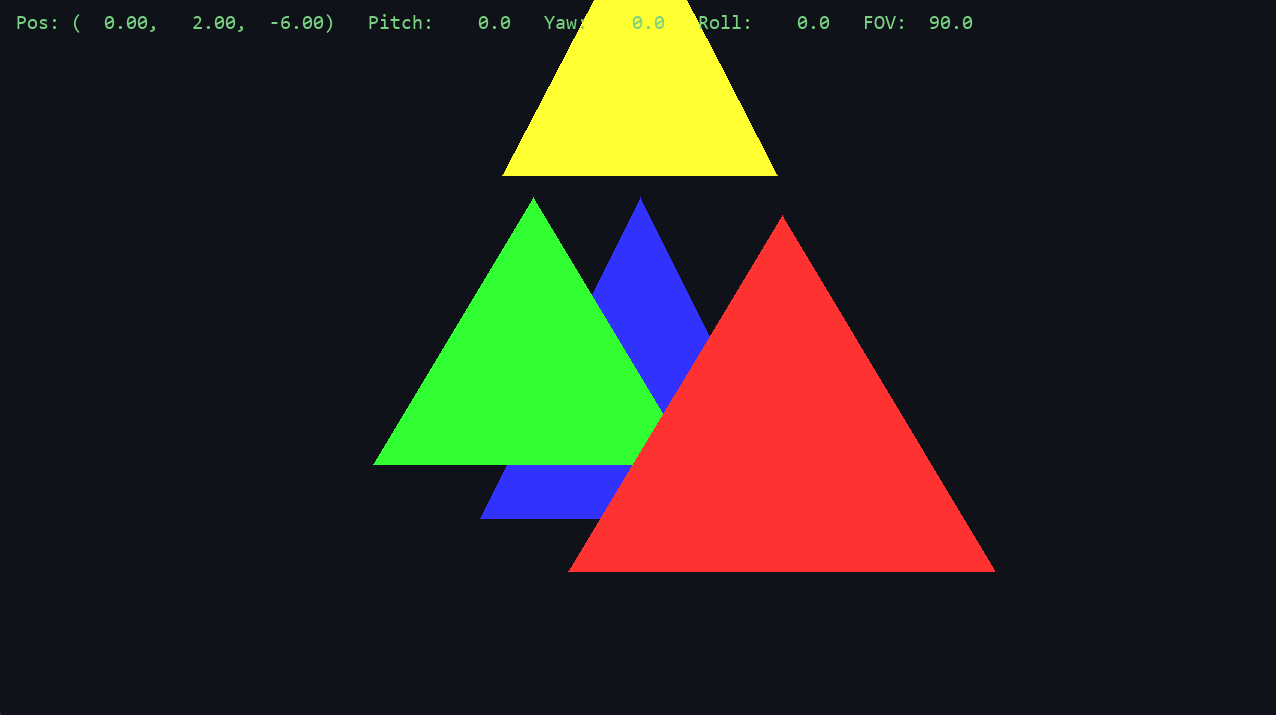
\includegraphics[width=0.8\textwidth]{screens/widokpoincicjacji.png}
    \caption{Scena 3D widziana frontalnie, tuż po uruchomieniu aplikacji.}
\end{figure}

\begin{figure}[H]
    \centering
    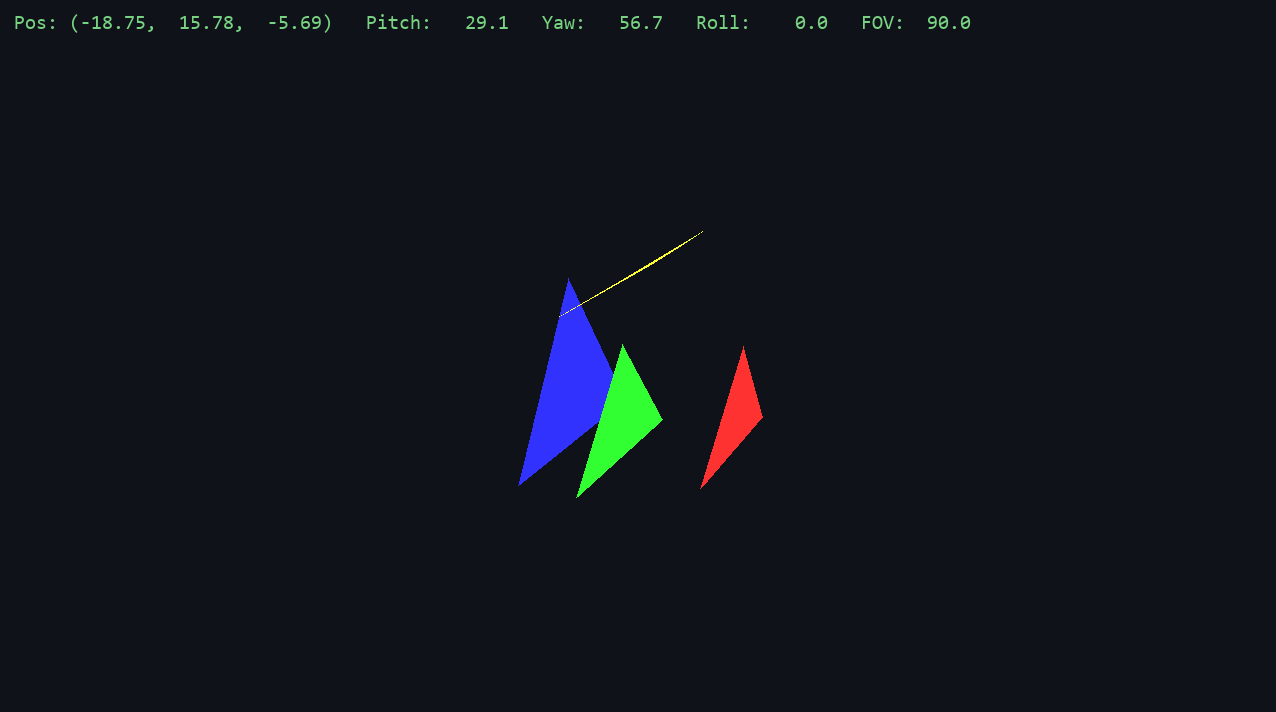
\includegraphics[width=0.8\textwidth]{screens/widokzgory.png}
    \caption{Układ wygenerowanych trójkątów na siatce współrzędnych - rzut na ułożenie obiektów w głębi sceny.}
\end{figure}
Zrzuty zamieszczone powyżej (Rysunek 1 oraz Rysunek 2) pełnią formę informacyjną wobec struktury mapy, pokazując tylko konstrukcję oraz ułożenie fizyczne użytych przedmiotów w bezpiecznej odległości i kolejności od Z. Pozwoli to z łatwością ocenić niżej umiejscowione zadania testowe.

\section{Testy działania}
Sprawdzaliśmy zachowanie programu głównie przez obracanie i przesuwanie kamery, obserwując, czy obiekty poprawnie zasłaniają się nawzajem.

\subsection{Test 1: Przysłonięcia przy rotacji kamery w lewo}
\textbf{Czynność:} Obrót kamery w lewo.
\\
\textbf{Oczekiwany efekt:} Niebieski trójkąt, który był dalej, pojawia się z przodu i zasłania elementy, które wcześniej były widoczne.

\begin{figure}[H]
    \centering
    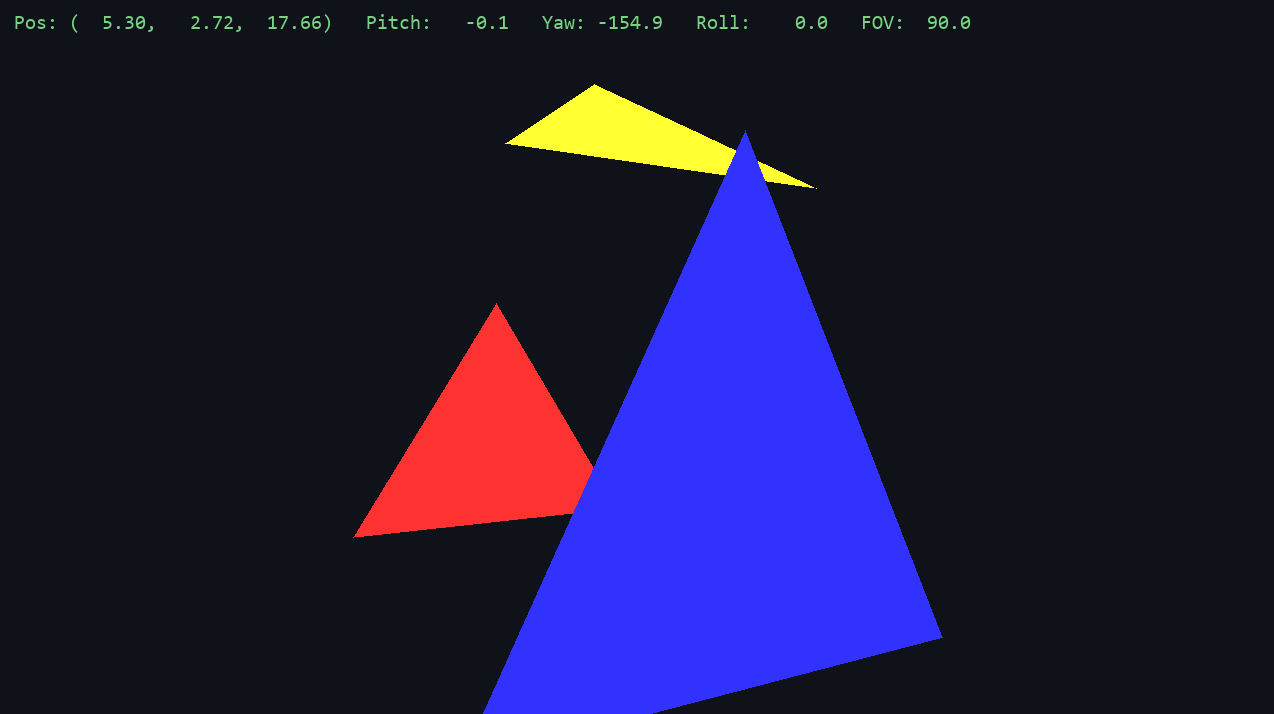
\includegraphics[width=0.8\textwidth]{screens/niebieskizaslaniazielonywpelni.png}
    \caption{Niebieski trójkąt prawidłowo przysłania widok z tyłu, blokując render elementu zielonego w osi wizualnej kamery.}
\end{figure}

\subsection{Test 2: Przysłonięcia przy rotacji kamery w prawo}
\textbf{Czynność:} Obrót kamery w prawo.
\\
\textbf{Oczekiwany efekt:} Widok się zmienia tak, że teraz zielony trójkąt może zasłaniać czerwony, zgodnie z nową perspektywą.

\begin{figure}[H]
    \centering
    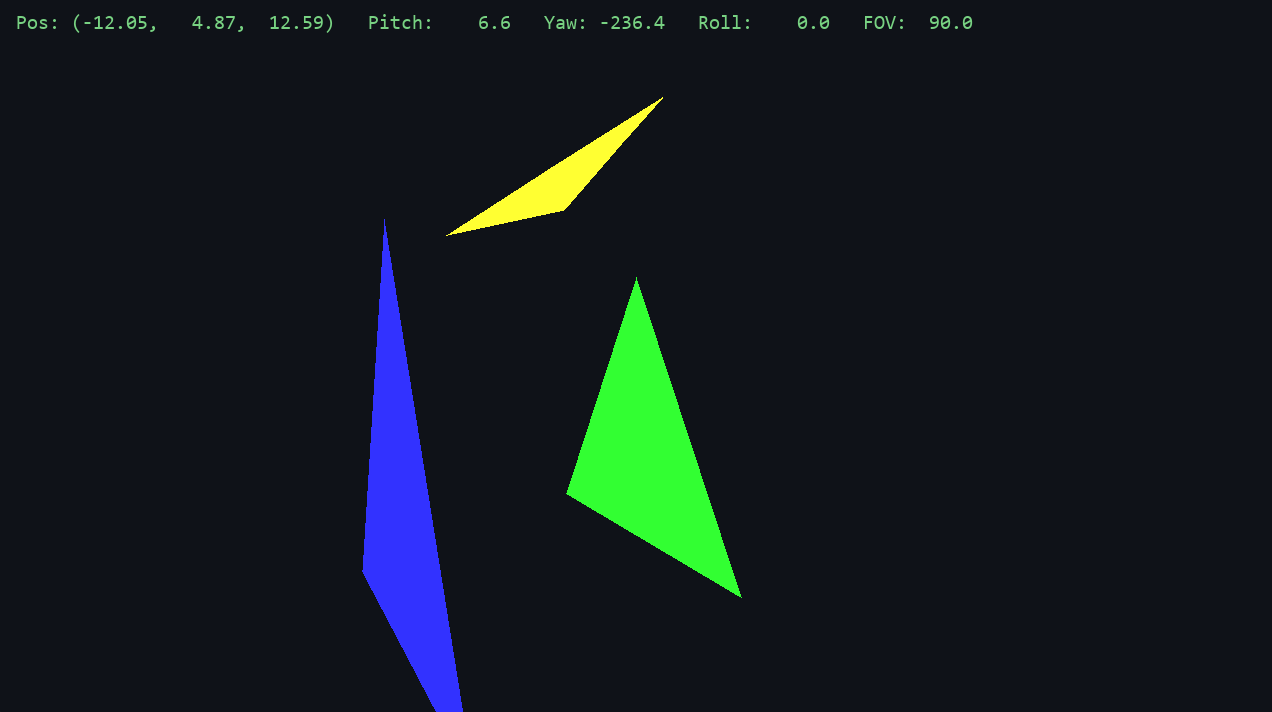
\includegraphics[width=0.8\textwidth]{screens/zielonyzaslaniaczerwonywpelni.png}
    \caption{Zamierzone zakrycie centralnego czerwonego przedmiotu odświeżającą zmianą perspektywy z prawej.}
\end{figure}

\subsection{Test 3: Okluzja elementu ukośnego (pochyłego)}
\textbf{Czynność:} Przesunięcie kamery w górę, by spojrzeć na żółty, pochyły trójkąt.
\\
\textbf{Oczekiwany efekt:} Żółty trójkąt zasłania fragmenty trójkątów pod nim, bez powstawania błędnych „wcięć” czy artefaktów.

\begin{figure}[H]
    \centering
    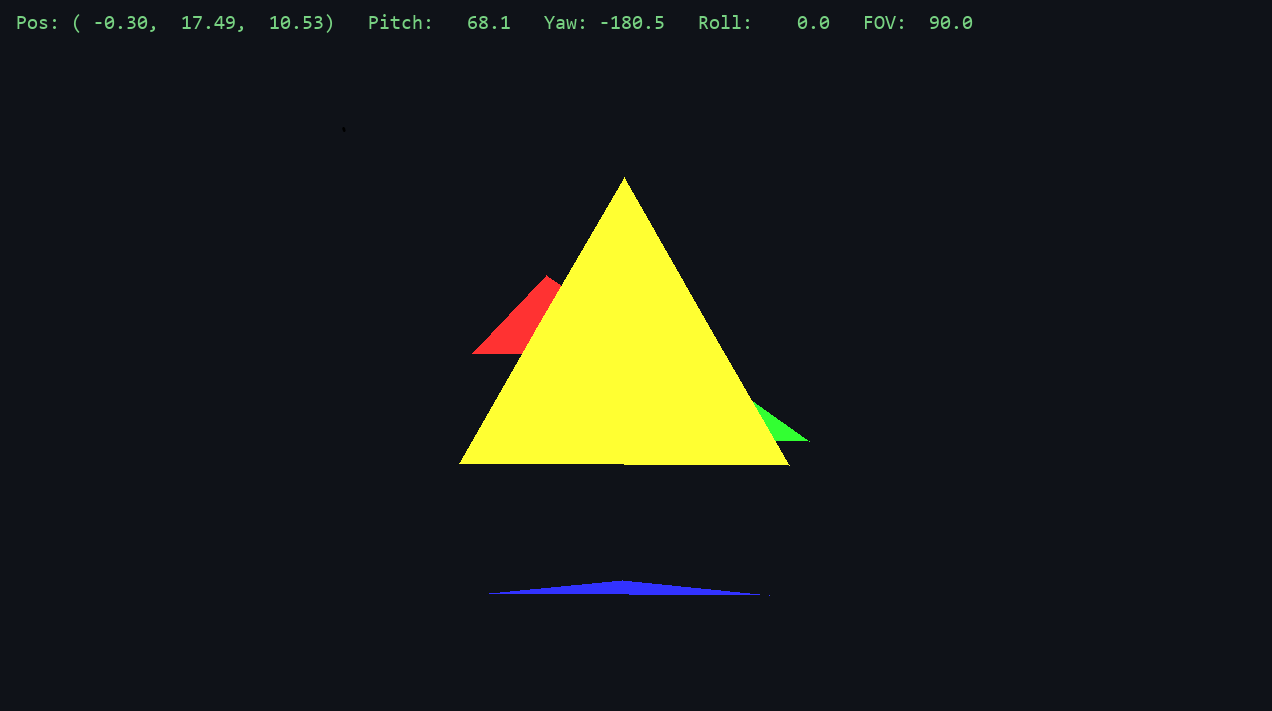
\includegraphics[width=0.8\textwidth]{screens/zoltyprzyslaniafragmentyzielonegoiczerwonego.png}
    \caption{Prawidłowe odcinanie rzutu brył pod pochyłym, skrajnym obiektem.}
\end{figure}

\section{Wnioski końcowe}
Drzewo BSP dobrze poradziło sobie z postawionym zadaniem. Dzięki niemu program potrafi posortować trójkąty od najdalszych do najbliższych, więc obiekty położone bliżej poprawnie zasłaniają te dalej. Rozwiązanie zadziałało efektywnie na naszej prostej scenie testowej i pozwoliło uniknąć używania kosztownego bufora Z. To prosty i szybki sposób na usuwanie zasłoniętych elementów, choć w bardzo złożonych scenach mogą być potrzebne dodatkowe poprawki.

\end{document}
